%%
%% This is file `sample-sigconf.tex',
%% generated with the docstrip utility.
%%
%% The original source files were:
%%
%% samples.dtx  (with options: `sigconf')
%% 
%% IMPORTANT NOTICE:
%% 
%% For the copyright see the source file.
%% 
%% Any modified versions of this file must be renamed
%% with new filenames distinct from sample-sigconf.tex.
%% 
%% For distribution of the original source see the terms
%% for copying and modification in the file samples.dtx.
%% 
%% This generated file may be distributed as long as the
%% original source files, as listed above, are part of the
%% same distribution. (The sources need not necessarily be
%% in the same archive or directory.)
%%
%% The first command in your LaTeX source must be the \documentclass command.
\documentclass[sigconf]{acmart}
\usepackage{booktabs}
\usepackage{graphicx, changepage}
\usepackage{CJKutf8} %for chinese
\usepackage[OT2,T1]{fontenc} %for russian
\usepackage{kotex} % korean

%%
%% \BibTeX command to typeset BibTeX logo in the docs
\AtBeginDocument{%
  \providecommand\BibTeX{{%
    \normalfont B\kern-0.5em{\scshape i\kern-0.25em b}\kern-0.8em\TeX}}}

%% Rights management information.  This information is sent to you
%% when you complete the rights form.  These commands have SAMPLE
%% values in them; it is your responsibility as an author to replace
%% the commands and values with those provided to you when you
%% complete the rights form.
\setcopyright{none}
\copyrightyear{2018}
\acmYear{2018}
\acmDOI{10.1145/1122445.1122456}

%% These commands are for a PROCEEDINGS abstract or paper.

\settopmatter{printacmref=false} % Removes citation information below abstract
\renewcommand\footnotetextcopyrightpermission[1]{} % removes footnote with conference information in first column
\pagestyle{plain} 
%%
%% Submission ID.
%% Use this when submitting an article to a sponsored event. You'll
%% receive a unique submission ID from the organizers
%% of the event, and this ID should be used as the parameter to this command.
%%\acmSubmissionID{123-A56-BU3}

%%
%% The majority of ACM publications use numbered citations and
%% references.  The command \citestyle{authoryear} switches to the
%% "author year" style.
%%
%% If you are preparing content for an event
%% sponsored by ACM SIGGRAPH, you must use the "author year" style of
%% citations and references.
%% Uncommenting
%% the next command will enable that style.
%%\citestyle{acmauthoryear}
%% remove the box 
\makeatletter
\def\runningfoot{\def\@runningfoot{}}
\def\firstfoot{\def\@firstfoot{}}
\makeatother 
%%
%% end of the preamble, start of the body of the document source.
\begin{document}

\makeatletter
\renewcommand\subsection{\@startsection{subsection}{3}{\z@}%
                                     {-3.25ex\@plus -1ex \@minus -.2ex}%
                                     {-1.5ex \@plus -.2ex}% Formerly 1.5ex \@plus .2ex
                                     {\normalfont\normalsize\bfseries}}
\makeatother

%%
%% The "title" command has an optional parameter,
%% allowing the author to define a "short title" to be used in page headers.
\title{Determining the cultural interpretation of minimalism in photography through the flickr database}

%%
%% The "author" command and its associated commands are used to define
%% the authors and their affiliations.
%% Of note is the shared affiliation of the first two authors, and the
%% "authornote" and "authornotemark" commands
%% used to denote shared contribution to the research.
\author{Marion Kramer}
\affiliation{%
  \institution{EPFL}
  \country{Switzerland}}
\email{marion.kramer@epfl.ch}

\author{Rémi Petitpierre}
\affiliation{%
  \institution{EPFL}
  \country{Switzerland}}
\email{remi.petitpierre@epfl.ch}

\author{Valentine Bernasconi}
\affiliation{%
  \institution{EPFL}
  \country{Switzerland}}
\email{valentine.bernasconi@epfl.ch}


%%
%% By default, the full list of authors will be used in the page
%% headers. Often, this list is too long, and will overlap
%% other information printed in the page headers. This command allows
%% the author to define a more concise list
%% of authors' names for this purpose.
\renewcommand{\shortauthors}{Petitpierre, et al.}

%%
%% The abstract is a short summary of the work to be presented in the
%% article.
\begin{abstract}
  The following paper attempts to determine the possible cultural impact on the interpretations of the artistic movement minimalism in photography. In order to determine the different trends within minimalism and to see if they are culturally specific, the flickr database was used. The corpus included 1'027'777 auto-tagged images, among which 4'356  images were also user-tagged and 193'153 were geolocalized. Based on these tags, the Louvain algorithm was applied to perform communities clustering. The outcome was 5 clusters representing different artistic trends: house and indoor activities, urban and geometry, landscapes, lights and nature.
\end{abstract}


%%
%% Keywords. The author(s) should pick words that accurately describe
%% the work being presented. Separate the keywords with commas.
\keywords{flickr, clustering, minimalism}

\settopmatter{printacmref=false}
%%
%% This command processes the author and affiliation and title
%% information and builds the first part of the formatted document.
%% remove the box 
\makeatletter
\def\@copyrightspace{\relax}
\makeatother
\maketitle

\section{Introduction}
Minimalism is a contemporary art movement born in the 60s and is still today widely used and applied, among other fields, in photography. The core idea of minimalistic photography is to capture simple lines or repetitive patterns, and restricted subjects and amount of colors. These simple guidelines easily offer a great place to different trends within the movement and might also vary according to different cultural contexts. Furthermore, the aspect of evolution of an artistic movement in time is not negligible, especially with the rise of new technologies and the change of our lifestyles and visual landscapes that occurred over the last 50 years.

Indeed, nowadays, artistic movements, such as minimalism, can benefit from greater exposures thanks to social media. The diversity of the platforms available, such as Instagram, Pinterest or Youpic, enable to easily share and explore similar content. Small and larger communities are thus established by these shared inspirations and trends are created, usually thanks to the use of tags or hashtags. In this era of globalisation, cross-cultural exchanges are more easily performed and the variety of possible expressions expand. However, do these trends still remain specific to a common culture or are they free from geographical boundaries?

On the social platform flickr, which allows professionals and non-professionals to share pictures and provide them with a variety of tags to connect with their piers, a strong community of minimalistic photographers exists. Grouped under tags such as \textit{'minimalis',  '{\fontencoding{OT2}\selectfont minimalism}', '\begin{CJK*}{UTF8}{gbsn}极简主义\end{CJK*}', '\begin{CJK*}{UTF8}{gbsn}ミニマリズム\end{CJK*}', '미니멀리즘'}, the pictures seem to embrace a great variety of possible interpretations of the movement. It is based on this community of tags that the project tries to establish the variety of existing trends in minimalism and to determine their possible correlations with cultural backgrounds based on the geo-location of the provided pictures. 

This paper first describes the dataset used from the Yahoo Flickr Creative Commons and the set of methods applied to the data. In order to determine the trends, tag-based clustering was used, followed by a set of classifiers to determine most relevant metadata and find a time and place dependence. In addition to this first range of work, image processing was performed to obtain more features based on the content of the images. Finally the results are discussed in section 4 and a conclusion is made.

\section{Data}
The data used in the context of the project is the Yahoo Flickr Creative Commons dataset that can be downloaded via the flickr api at \url{https://www.flickr.com/services/api/}. Each image contains a photo\_id, a jpeg url, a title, a description, a camera type and tags. The corpus thus includes 1'027'777 auto-tagged images, among which 4'356  images are also user-tagged and 193'153 are geolocalized. The dataset also contains time information 99,99\% of the time.

%\subsection{Template Styles}

%The primary parameter given to the ``\verb|acmart|'' document class is
%the {\itshape template style} which corresponds to the kind of publication
%or SIG publishing the work. This parameter is enclosed in square
%brackets and is a part of the {\verb|documentclass|} command:
%\begin{verbatim}
  %\documentclass[STYLE]{acmart}
%\end{verbatim}

%Journals use one of three template styles. All but three ACM journals
%use the {\verb|acmsmall|} template style:
%\begin{itemize}
%\item {\verb|acmsmall|}: The default journal template style.
%\item {\verb|acmlarge|}: Used by JOCCH and TAP.
%\item {\verb|acmtog|}: Used by TOG.
%\end{itemize}

%The majority of conference proceedings documentation will use the {\verb|acmconf|} template style.
%\begin{itemize}
%\item {\verb|acmconf|}: The default proceedings template style.
%\item{\verb|sigchi|}: Used for SIGCHI conference articles.
%\item{\verb|sigchi-a|}: Used for SIGCHI ``Extended Abstract'' articles.
%\item{\verb|sigplan|}: Used for SIGPLAN conference articles.
%\end{itemize}


\section{Methods}
\subsection*{Tag-based clustering.}
\subsection*{Classifying relevant metadata.}
\subsection*{Classifying for time and place dependence.}
\subsection*{Image processing.}
\section{Results}
From the very first steps of data processing, our understanding of minimalism grew and we were able to realize that minimalism is a way of perceiving a surrounding environment and that no specific subject requires to be created for the purpose of a minimalistic picture. Indeed, the content of the tags indicate a great variety of image contents, from indoor to outdoor topics. Furthermore, minimalism appears to be mostly prevalent in western Europe and the USA's East and West coasts. Regarding other continents, the movement appears to be more used in touristic places, mainly national parks, and in large cities rather than in rural environments.
\begin{figure}[h]
 		 \centering
 			 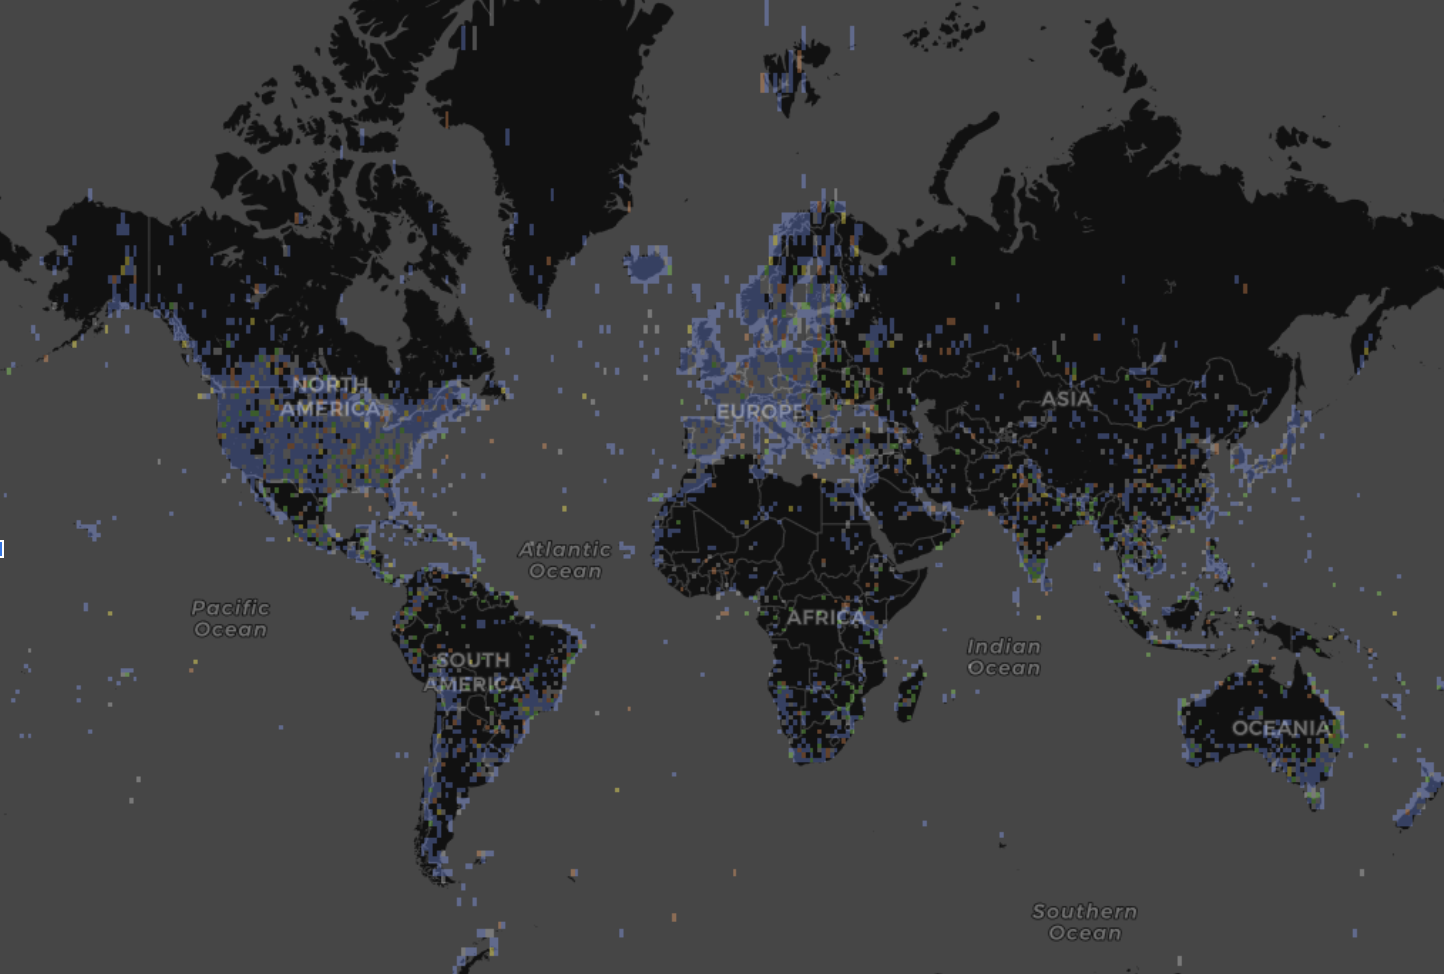
\includegraphics[width=\linewidth]{images/data_trends}
 			 \caption{data trends and spacial representations}
	\end{figure}
\subsection*{Trends in minimalism.}
Out of the first clustering performed on the tags, 5 major trends were outlined.
	\begin{itemize}
		\item Indoor related activities: home, food
		\item Urban environments
		\item Lights
		\item Landscapes, sky and sea
		\item Nature (macro pictures)
	\end{itemize}
However, based on the maps generated from these clusters, none of these five trends seem to belong to a specific region of the world. Although no direct correlation can be drew between a trend and a culture, we can see tendencies. Urban and lights content correspond to major urban centres located in Asia's and USA's East coasts and Europe. Landscapes, on the other hand, are more equally spread among the different continents and are especially focused on coasts, due to the dominance of sea views. Nature is more dominant in wooded regions, such as wildlife sanctuaries, nature reserves and national parks. 

Thereby, if minimalism is not related to a culture, it can be still considered as a way of expressing a certain lifestyle.

\section{Conclusions}

\section{Appendix}

%%
%% The next two lines define the bibliography style to be used, and
%% the bibliography file.
\bibliographystyle{ACM-Reference-Format}
\bibliography{sample-base}

%%
%% If your work has an appendix, this is the place to put it.
\appendix


\section{Online Resources}

Nam id fermentum dui. Suspendisse sagittis tortor a nulla mollis, in
pulvinar ex pretium. Sed interdum orci quis metus euismod, et sagittis
enim maximus. Vestibulum gravida massa ut felis suscipit
congue. Quisque mattis elit a risus ultrices commodo venenatis eget
dui. Etiam sagittis eleifend elementum.

Nam interdum magna at lectus dignissim, ac dignissim lorem
rhoncus. Maecenas eu arcu ac neque placerat aliquam. Nunc pulvinar
massa et mattis lacinia.

\end{document}
\endinput
%%
%% End of file `sample-sigconf.tex'.
